\section{Results}

Two sets of data were taken, and are examined here in terms of the accuracy of
their produced models and the possible causes of error in the reconstruction
process. The first set of photographs were taken at Long Ashton Farm outside
Bristol, and the second set were taken at the Avon Gorge in Bristol.

\subsection{Long Ashton}

For this data set, a hexacopter was used to gather a total of 63 aerial images.
The time interval technique was used to take the photos, and the time offset
method used to geotag the resulting photos.

\subsubsection{Without GCPs}

Firstly, the reconstruction was run without the Ground Control Points input, and
without any photographic alignment optimisation. The resulting orthophoto is
shown in Figure \ref{img:long-ashton/no-gcp/orthophoto}, while the DEM is shown
in Figure \ref{img:long-ashton/no-gcp/dem}.

\begin{figure}
    \centering
    \begin{subfigure}[b]{0.49\textwidth}
        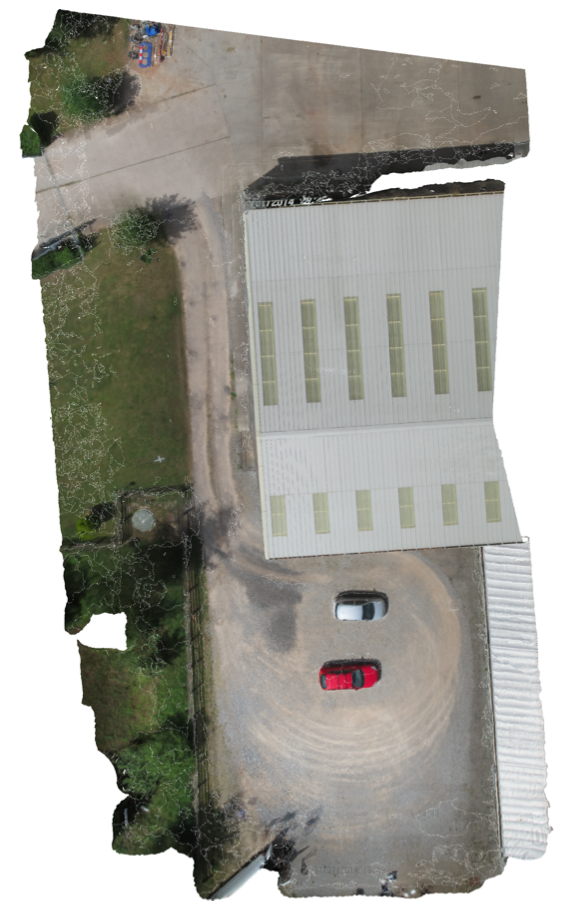
\includegraphics[width=0.5\textwidth]{LongAshtonNoGCPOrthophoto}
        \caption{The generated orthophoto for the Long Ashton data set, without
        GCPs input.}
        \label{img:long-ashton/no-gcp/orthophoto}
    \end{subfigure}
    \begin{subfigure}[b]{0.49\textwidth}
        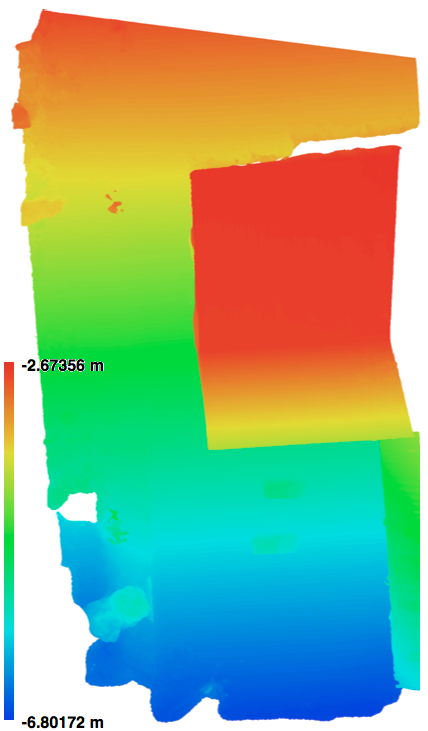
\includegraphics[width=0.5\textwidth]{LongAshtonNoGCPDEM}
        \caption{The generated DEM for the Long Ashton data set, without GCPs
        input.}
        \label{img:long-ashton/no-gcp/dem}
    \end{subfigure}
\end{figure}

\subsection{Avon Gorge}

\subsection{Ground Control Point Accuracy}

Which GCPs produced the biggest errors and why. Sources of stated errors in
PhotoScan generated report.

\subsection{Model and DEM Analysis}

\begin{itemize}

    \item PhotoScan calculated meters per pixel.

    \item Error - find out where PhotoScan calculates this from!

    \item Photographics overlap

\end{itemize}
